\documentclass[conference,a4paper]{IEEEtran}
\usepackage{kotex}
\usepackage{amsmath,amssymb,bm}
\usepackage{graphicx,booktabs,array}
\usepackage{cite}
\usepackage[hidelinks,unicode]{hyperref}
\usepackage{url}
\setmainfont{texgyretermes-regular.otf}[
 BoldFont=texgyretermes-bold.otf,
 ItalicFont=texgyretermes-italic.otf,
 BoldItalicFont=texgyretermes-bolditalic.otf]
\setsansfont{texgyreheros-regular.otf}[
 BoldFont=texgyreheros-bold.otf,
 ItalicFont=texgyreheros-italic.otf,
 BoldItalicFont=texgyreheros-bolditalic.otf]
\renewcommand{\abstractname}{초록}
\renewcommand{\IEEEkeywordsname}{주요어}
\renewcommand{\refname}{참고문헌}
\renewcommand{\figurename}{그림}
\renewcommand{\tablename}{표}
\newcommand{\R}{\mathbb{R}}
\newcommand{\norm}[1]{\left\lVert#1\right\rVert}
\newcommand{\wrap}{\operatorname{wrap}}
\graphicspath{{figures/}}
\hypersetup{pdftitle={예측 정확도와 인계 성공의 관계: 학습 동역학 기반 부품 밀기 계획의 통제 비교},pdfauthor={codemillss}}

\begin{document}
\title{예측 정확도와 인계 성공의 관계:\\학습 동역학 기반 부품 밀기 계획의 통제 비교\\
\large From Prediction Accuracy to Handoff Success:\\A Controlled Study of Learned Dynamics for Planar Pushing}
\author{\IEEEauthorblockN{codemillss}}
\maketitle

\begin{abstract}
학습 동역학의 예측오차 감소가 로봇의 행동 선택과 작업 성공을 개선하는지는 별도의 검증이 필요하다.
본 연구는 단일 직사각형 부품의 밀기 정렬에서 한 단계 전이 학습(S1)과 다단계 자유 예측 손실을 추가한 학습(SK)을 비교한다.
상태·행동 표현, 출발 가중치, Adam 상태, 자료, 배치 순서 및 추가 갱신 수를 통제하고, 고정 행동의 예측, 동일 후보의 선택, 폐루프 인계를 분리하여 평가하였다.
12개 독립 초기조건에서 96회 폐루프 실행을 수행하고, 그중 6개 초기조건에서 추출한 12개 상태에서 후보별 실제 미래를 576회 실행하였다.
기하 피드백, 선형 모델 계획, S1 및 SK의 인계 성공은 각각 8/12, 0/12, 13/36 및 12/36이었다.
일부 학습 seed에서 SK의 5·10단계 위치 예측오차가 감소했으나, 인계 성공 개선은 확인되지 않았다
(S1 대비 $-2.78$ percentage points, 95\% family bootstrap 구간 $[-8.33,0.00]$).
동일 상태·후보 진단에서 S1과 SK는 36쌍 중 35쌍에서 같은 후보를 선택하였다.
결과는 제한된 고정 행동의 예측 개선이 후보 선택과 인계 성과의 충분조건이 아님을 보여준다.
비용 정합성, 방문 상태 분포 및 복구 후보의 제약은 가능한 설명이지만 최종 실패의 단일 원인으로 분리되지는 않았다.
\end{abstract}
\begin{IEEEkeywords}
학습 동역학, 모델 예측 제어, 평면 밀기, 다단계 예측, 폐루프 평가
\end{IEEEkeywords}

\section{서론}\label{sec:intro}
부품 공급·취급 시스템에서는 후속 로봇이 사용할 수 있도록 부품의 위치와 방향을 유지하는 과정이 필요할 수 있다.
실제로 소형 부품을 전용 툴링·트랙·셔틀로 정렬하여 공급한 사례가 공개되어 있다~\cite{fortville2022}.
그러나 이러한 작업의 존재가 학습 모델이나 별도 밀기 정렬의 필요성을 의미하지는 않는다.
고정 지그, 피더, 현재 자세에서의 직접 집기 및 기하 피드백도 유효한 대안이다.
본 연구는 현장 도입 효과를 추정하기보다, 인계 자세 정렬이라는 구체적 작업에서 학습 예측이 의사결정에 전달되는 과정을 검증한다.

학습 동역학을 계획에 사용하는 방법은 이미 연구되어 왔다~\cite{bauza2018,chua2018}.
학습 목적과 제어 목적이 다르므로 예측 점수만으로 작업 성능을 판단하기 어렵다~\cite{lambert2020}.
평균 오차가 감소하더라도 후보 비용 순위가 바뀌지 않거나 자체 정책의 방문 상태에서 오차가 증가하면 폐루프 결과는 개선되지 않을 수 있다.
본 연구의 질문은 \emph{동일 모델 계열에 자유 예측 손실을 추가할 때 고정 행동 예측, 후보 선택 및 실제 인계는 각각 어떻게 변하는가?}이다.

이를 위해 작은 신경망의 행동 조건부 증분 모델을 구현하고 한 단계·다단계 학습을 통제 비교하였다.
평가는 (i) 공통 실제 행동열의 재귀 예측, (ii) 고정 상태·후보에서의 실제 비용 대조, (iii) 각 방법의 폐루프 인계로 구성된다.
기여는 새 제어 알고리즘이 아니라 이 세 평가를 연결한 제한된 조건의 실증 비교와 실패 분석이다.
공개 코드·모델·선별 결과~\cite{repository}를 통해 예측 개선과 작업 개선을 분리하여 검토할 수 있도록 하였다.

\section{관련 연구}\label{sec:related}
\subsection{평면 밀기와 학습 동역학}
Yu 등은 표면 재질, 형상, 접촉 위치, 밀기 방향·속도·가속도를 변화시킨 실물 자료를 수집하고 마찰과 모델 가정을 분석하였다~\cite{yu2016}.
본 연구는 형상·물성을 고정한 시뮬레이션이므로 해당 실물 변동이나 범용 접촉 조작을 재현하지 않는다.
Bauza 등은 Gaussian process 동역학을 선형화한 MPC와 제약 조건을 결합하였다~\cite{bauza2018}.
본 연구는 결정론적 MLP와 유한 후보 탐색을 사용하며 해당 방법의 직접 재현이나 성능 비교를 목적으로 하지 않는다.

\subsection{예측 목적과 제어 목적}
Chua 등은 확률적 신경망 앙상블과 불확실성 전파를 결합한 PETS를 제안하였다~\cite{chua2018}.
본 결정론적 모델에는 앙상블·확률적 불확실성 전파·온라인 자료 확장이 포함되지 않는다.
Lambert 등은 한 단계 예측 학습과 하위 제어 성능 사이의 목적 불일치를 지적하였다~\cite{lambert2020}.
본 연구는 그 문제의 일반적 해결책을 제안하지 않고 다단계 손실의 효과를 예측·선택·인계로 나누어 관찰한다.
따라서 알려진 현상의 일반적 신규성과 이번 부품 밀기 조건의 실증 관찰을 구분한다.

\begin{figure*}[t]
\centering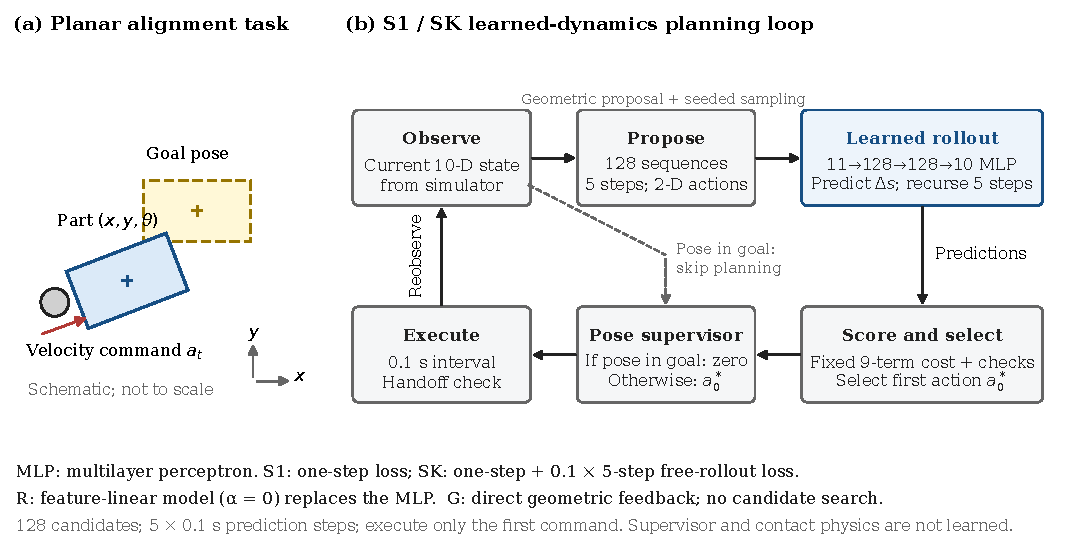
\includegraphics[width=\textwidth]{method_system.pdf}
\caption{실험 과제와 제어 구조의 개념도. 학습 모델은 상태 증분을, 계획기는 예측 비용에 따른 후보 선택을 담당한다.
접촉 물리와 속도 추종은 시뮬레이터·기존 서보가, 목표 자세 안의 영 명령과 유지 판정은 공통 감독기가 담당한다.
실험 사진이나 실제 예측 궤적을 그린 그림은 아니다.}\label{fig:system}
\end{figure*}

\section{문제 정식화}\label{sec:problem}
\subsection{상태와 행동}
관측 상태를
\begin{equation}
s_t=[p_t^o,\theta_t,v_t^o,\omega_t,p_t^p,v_t^p]\in\R^{10}
\label{eq:state}
\end{equation}
으로 정의한다.
$p^o,p^p,v^o,v^p\in\R^2$는 부품·푸셔의 world XY 위치와 속도이고 $\theta,\omega$는 부품 yaw와 각속도이다.
행동 $u_t\in\R^2$는 $\Delta t=0.1\,\mathrm{s}$ 동안 유지하는 목표 속도이다.
유한한 힘으로 추종하므로 $u_t$와 실제 푸셔 속도는 같지 않을 수 있다.
현재 상태는 시뮬레이터에서 직접 읽으며 카메라 추정은 사용하지 않는다.
3차원 자유 강체를 평면 관측으로 표현하므로 식~\eqref{eq:state}의 충분통계성을 보장하지 않는다.

\subsection{인계 성공}
목표는 $(p^\star,\theta^\star)=((0.08,0),0)$이며, 직사각형의 $\pi$ 대칭 방향 오차는
\begin{equation}
e_\theta(s)=\tfrac12\operatorname{atan2}
\big(\sin 2(\theta-\theta^\star),\cos 2(\theta-\theta^\star)\big)
\label{eq:yaw}
\end{equation}
이다.
위치 오차 norm, $|e_\theta(s)|$, 선속도 norm, 각속도 절댓값이 각각 $5\,\mathrm{mm}$, $3^\circ$,
$0.01\,\mathrm{m/s}$, $0.05\,\mathrm{rad/s}$ 이하인 상태를 $\chi(s)=1$로 둔다.
성공은 최대 $30\,\mathrm{s}$ 이내 행동 경계에서 직전 $0.3\,\mathrm{s}$의 모든 물리 표본이 $\chi=1$을 만족한 경우다.
표본 간격은 $0.5\,\mathrm{ms}$이며 연속 시간 전체의 해석적 보장을 뜻하지 않는다.
이는 후속 인계 조건으로 설정한 실험 명세이며 산업 공차나 실제 집기 성공률이 아니다.
작업 재시도는 허용하지 않는다.

\section{방법}\label{sec:method}
\subsection{행동 조건부 증분 모델}
입력 특징은
\begin{equation}
\phi(s_t,u_t)=[p_t^p-p_t^o,\sin2\theta_t,\cos2\theta_t,
v_t^o,\omega_t,v_t^p,u_t]\in\R^{11}
\label{eq:feature}
\end{equation}
이다.
Train 평균·대각 scale을 $\mu_x,D_x,\mu_\Delta,D_\Delta$라 하면,
\begin{align}
\widehat{\Delta s}_t&=\mu_\Delta+D_\Delta
 f_\psi\!\left(D_x^{-1}(\phi(s_t,u_t)-\mu_x)\right),\label{eq:model}\\
\hat s_{t+1}&=s_t\oplus\widehat{\Delta s}_t \label{eq:integrate}
\end{align}
로 다음 상태를 얻는다.
$\oplus$는 성분별 덧셈 후 yaw를 $[-\pi,\pi)$로 감싼다.
Raw yaw 증분의 절댓값이 $\pi$ 이상이면 적분 전에 무효로 처리한다.
푸셔를 포함한 전체 예측 상태를 재입력하고 목표 자세는 비용에 사용한다.

$f_\psi$는 $11$--$128$--$128$--$10$ 구조, 두 SiLU 은닉층과 선형 출력의 MLP로 19,338개 파라미터를 갖는다.
모델은 float32, 물리 경계와 정규화 통계는 float64다.
정규화는 겹치는 창을 중복 집계하지 않고 train 원전이로만 적합한다.
Scale은 모집단 표준편차와 성분별 하한 중 큰 값이며 sin/cos 특징은 평균 0·scale 1로 고정한다.

\subsection{한 단계 및 다단계 학습}
$\delta(a,b)$를 yaw 성분만 $2\pi$ wrap한 $b-a$라 하자.
창 $i$의 유효 전이 mask $m_{ik}$와 $M=\sum_{i,k}m_{ik}$를 사용하며,
$\Delta s_{ik}=\delta(s_{ik},s_{i,k+1})$에 대한 손실은
\begin{equation}
\mathcal L_{\rm one}=
\frac{1}{10M}\sum_{i,k}m_{ik}
\norm{D_\Delta^{-1}\delta\!\left(
\Delta s_{ik},\widehat{\Delta s}(s_{ik},u_{ik})\right)}^2
\label{eq:one}
\end{equation}
이다.
S1도 $K=5$ 창 안의 실제 전이 다섯 개를 모두 사용한다.
자유 예측은 $\hat s_{i0}=s_{i0}$에서 식~\eqref{eq:model}--\eqref{eq:integrate}를 재귀 적용하고,
\begin{equation}
\mathcal L_{\rm roll}=
\frac{1}{10M}\sum_i\sum_{k=1}^{K}m_{i,k-1}
\norm{D_\Delta^{-1}\delta(s_{ik},\hat s_{ik})}^2
\label{eq:roll}
\end{equation}
를 계산한다.
미래 실제 상태는 정답과 한 단계 항에만 사용한다.
두 방법은
\begin{align}
\mathcal L_{\rm S1}&=\mathcal L_{\rm one},\nonumber\\
\mathcal L_{\rm SK}&=\mathcal L_{\rm one}+0.1\mathcal L_{\rm roll}
\label{eq:objectives}
\end{align}
로 구분된다.
종료 뒤 padding은 제외하되 예측 실패를 사후 mask로 제거하지 않는다.
S1에는 자유 예측 forward가 없으므로 동일 갱신 수는 동일 FLOPs가 아니다.

\subsection{유한 후보 기반 계획}
매 시점 $N=128$개의 $H=5$ 명령열을 만들며, 길이 2와 3의 두 상수 블록으로 표현한다.
예약 후보 8개, 전역 후보 60개, 기하 제안 주변 30개, 이전 계획 주변 30개를 사용하고 명령 norm은 $0.03\,\mathrm{m/s}$ 이하이다.
난수 키에서 모델 ID와 학습 seed는 제외하지만, 기하 제안과 warm start가 상태·이력에 의존하므로 폐루프 전체 후보 배열이 방법마다 같지는 않다.

Post-action 상태에서 $P_k=\norm{\hat p^o_{t+k}-p^\star}/0.005$,
$A_k=e_\theta(\hat s_{t+k})/(3^\circ)$로 둔다.
후보의 $k$번째 명령을 $a_k$, 직전 실제 명령을 $a_0$라 하면,
\begin{align}
U_k&=\norm{a_k/0.06}^2,\quad
V_k=\norm{(a_k-a_{k-1})/0.06}^2,\nonumber\\
G_k&=\big(\max(d(\hat s_{t+k}),0)/0.08\big)^2 \label{eq:terms}
\end{align}
이며 $d$는 회전 직사각형 signed distance에서 푸셔 반지름을 뺀 간격이다.
최종 비용은
\begin{align}
J={}&\Delta t\sum_{k=1}^{H}
\big(P_k^2+A_k^2+0.02U_k+0.02V_k+0.1G_k\big)\nonumber\\
&+5P_H^2+5A_H^2
+0.1\left(\frac{\norm{\hat v_H^o}}{0.01}\right)^2
+0.1\left(\frac{\hat\omega_H}{0.05}\right)^2 .
\label{eq:cost}
\end{align}
탐색 범위와 달리 명령 비용 scale은 물리 한계 $0.06\,\mathrm{m/s}$다.
비유한 상태·작업 공간 이탈·$1\,\mathrm{mm}$ 초과 예측 침투 등의 무효 비용은 $\infty$이며, 유효 후보가 없으면 계획 실패로 종료한다.
동률은 낮은 후보 번호를 선택한다.
첫 $0.1\,\mathrm{s}$만 실행하고 재관측하며, 계획 중 실제 미래 물리를 조회하지 않는다.
실제 위치·방향이 목표 안이면 공통 감독기가 영 명령을 적용해 정지·유지를 검사한다.
따라서 인계 성과는 계획·서보·감독기의 결합 결과다(그림~\ref{fig:system}).

\section{실험 설정}\label{sec:experiments}
\subsection{환경 및 자료}
MuJoCo~\cite{mujoco}에서 단일 부품과 원형 푸셔의 마찰 접촉을 실행하였다.
주요 조건은 표~\ref{tab:settings}와 같다.
바닥--부품 sliding friction 계수는 $(0.3,0.3)$, 푸셔--부품은 $(0.5,0.5)$로 고정하였다.
Apple Silicon CPU에서 Python 3.14.7, NumPy 2.5.3, PyTorch 2.14.0, MuJoCo 3.14.0을 사용하였다.

\begin{table}[t]
\caption{고정 실험 조건}\label{tab:settings}
\centering\small
\begin{tabular}{@{}ll@{}}
\toprule 항목 & 값\\ \midrule
부품 크기 / 질량 & $80\times60\times20\,\mathrm{mm}$ / $0.1\,\mathrm{kg}$\\
푸셔 반지름 / 질량 & $8\,\mathrm{mm}$ / $0.1\,\mathrm{kg}$\\
속도 서보 이득 / 힘 한계 & $20\,\mathrm{N\,s/m}$ / $\pm2\,\mathrm N$\\
물리 / 행동 간격 & $0.0005\,\mathrm s$ / $0.1\,\mathrm s$\\
적분기 / 접촉 cone & implicitfast / elliptic\\
후보 / horizon & $128$ / $5$ ($0.5\,\mathrm s$)\\
위치 / 방향 허용오차 & $5\,\mathrm{mm}$ / $3^\circ$\\
선속도 / 각속도 허용값 & $0.01\,\mathrm{m/s}$ / $0.05\,\mathrm{rad/s}$\\
유지 / 제한 시간 & $0.3\,\mathrm s$ / $30\,\mathrm s$\\
\bottomrule
\end{tabular}
\end{table}

수집 전에 초기조건 family 단위로 train과 validation을 분리하였다.
비접촉, 중앙 밀기, 편심 밀기, 접촉 전환, 기하 피드백 및 교란 기하 피드백의 여섯 모드를 사용했다.
Train 60개 family의 3,200전이, validation 30개 family의 1,600전이가 모두 유효했다.
K5 겹침 창은 각각 2,960개와 1,480개이며 독립 실험 수로 세지 않는다.

\subsection{기준선과 학습 통제}
방법은 조정된 기하 피드백(G), 선형 증분 예측과 공통 계획기(R), S1 및 SK다.
R은 Ridge 계열에서 선정한 $\alpha=0$의 선형 회귀다.
R·S1·SK는 식~\eqref{eq:cost}와 계획 규칙을 공유한다.
G는 제어 구조가 다르므로 G와 MLP의 차이를 신경망만의 효과로 귀속하지 않는다.

Seed는 11, 23, 47이다.
공통 MLP는 새 가중치와 Adam, 학습률 $10^{-3}$, batch 256으로 100 epoch 학습하고,
validation의 K5 끝점 점수로 각각 epoch 100, 97, 98을 선정하였다.
각 seed의 S1/SK는 동일 가중치, Adam 모멘트·step, 정규화, Torch·shuffle RNG와 배치 순서에서 분기하여
batch 64의 K5 창으로 각각 1,000 update를 추가했다.
Weight decay는 0, gradient clip norm은 1이다.
SK의 가중치는 $\{0.1,1.0\}$ 중 최종 validation 점수의 seed 평균으로 공통 선정하였다.
Validation은 공통 체크포인트·가중치 선정에 재사용되며, 최종 결과로 조정하지 않았다.
최종 비교에는 추가 update 1,000을 사용했다.
선정 점수는 K5 끝점의 위치오차$/5\,\mathrm{mm}$와
$|2\pi\text{-wrap yaw 잔차}|/(3^\circ)$의 합을 첫 전이 접촉 3군별로 평균한 뒤 동일 가중 평균한 값이다.
무효 K5 창이나 누락 접촉군이 있으면 선정 부적격이다.

\subsection{분리된 평가}
\emph{고정 행동 예측:}
G의 12개 실제 경로에서 실제 현재 상태와 적용 명령을 고정하고 $K=1,5,10$ 자유 예측을 평가했다.
실제 적격 창은 2,656/2,608/2,548개이고 종료 경계 제외는 0/48/108개다.
예측 무효를 별도 보고하고 family별 조건부 평균을 12개 family에 동일 가중 평균하였다.

\emph{후보 선택(E1):}
각 층 첫 두 family의 G tick 0과 29, 총 12상태에서 후보 16개를 고정했다.
후보별 실제 미래 3회로 $12\times16\times3=576$회, 2,880개 행동 구간을 얻었다.
7개 모델이 같은 실제 라벨을 공유하여 84개 진단 집합을 구성했고 독립 family는 6개다.
세 반복 모두 유효한 후보 집합을 $\mathcal V$라 하면,
\begin{equation}
\ell_{\rm sel}=\bar J_{\hat j}-\min_{j\in\mathcal V}\bar J_j,
\qquad \hat j=\arg\min_j\widehat J_j
\label{eq:selection}
\end{equation}
로 선택손실을 정의한다.
$\bar J_j$는 실제 비용 3회 평균이다.
이는 유한 후보군 비교이며 전역 최적 제어와의 차이가 아니다.
반복 범위가 겹치는 순위는 구별 보류로 남기고 그 범위를 신뢰구간으로 해석하지 않는다.

\emph{폐루프 인계(E2):}
병진·회전·접촉 위치 오프셋 각 4개 family, 총 12조건에서 G·R 및 S1/SK의 세 seed를 실행했다.
전체는 96회, MLP당 36회는 12개 독립 family와 3개 seed의 조합이다.
Timeout과 계획·제어 실패도 분모에 남긴다.
학습 손실 효과(E3)는 E1/E2를 재사용하며 새 실행 수를 추가하지 않는다.

\subsection{통계 및 복구 절차}
E2에서 방법 $m$, family $f$의 seed 평균 성공을 $q_{mf}$라 하면 방법 차이는
$12^{-1}\sum_f(q_{af}-q_{bf})$이다.
층 내 family를 복원 추출한 bootstrap 2,000회(seed 7711)의 95\% percentile 구간을 사용했다.
E1은 family 내 두 tick 및 학습 seed를 먼저 평균한 뒤 층당 2개, 총 6개 family를 같은 층화 방식으로 bootstrap하였다.
후보·물리 반복·겹치는 창·seed를 추가 독립 family로 세지 않았다.
탐색적 비교이며 다중비교 보정은 하지 않았다.

첫 정식 실행은 R 제어 후 저장 과정에서 중단되었다.
원본을 보존하고 저장기만 보완하여 같은 초기조건·모델·비용·계획으로 새 실행을 수행했다.
부모 결과를 합치거나 유리한 결과로 교체하지 않았다.
일부 결과를 이미 알게 된 동일 조건의 복구 평가이므로 새로운 blind holdout은 아니다.
분석은 행 순서를 고정해 원래 요약과 bootstrap 배열을 재생성했다.

\section{결과}\label{sec:results}
\subsection{고정 행동 예측}
표~\ref{tab:prediction}은 위치 예측오차다.
Seed 23·47은 두 모델이 모든 적격 창에서 유효하여 공통 모집단의 기술적 비교가 가능했다.
두 seed에서 SK의 K5·K10 오차가 낮았다(그림~\ref{fig:prediction}).
R의 K1/K5/K10 예측 무효는 47/358/627개, S1-11은 0/2/2개이고 다른 MLP는 0개다.
R 또는 seed11의 유효 창 평균만으로 같은 모집단의 개선을 주장하지 않는다.
독립 family는 12개이며 겹치는 창은 독립 표본이 아니다.

\begin{table}[t]
\caption{고정 행동 위치 예측오차 (mm).
Family 우선 조건부 평균; $^\dagger$는 유효 mask가 다른 모델.}\label{tab:prediction}
\centering\small
\begin{tabular}{@{}lrrr@{}}
\toprule 모델 & K1 & K5 & K10\\ \midrule
R$^\dagger$ & 0.0965 & 0.8695 & 1.6056\\
S1-11$^\dagger$ & 0.0206 & 0.0871 & 0.1562\\
SK-11 & 0.0226 & 0.0881 & 0.1514\\
S1-23 & 0.0204 & 0.0906 & 0.1669\\
SK-23 & 0.0175 & 0.0586 & 0.0957\\
S1-47 & 0.0193 & 0.0842 & 0.1475\\
SK-47 & 0.0189 & 0.0690 & 0.1083\\ \midrule
실제 적격 창 & 2,656 & 2,608 & 2,548\\
R 유효 창 & 2,609 & 2,250 & 1,921\\
S1-11 유효 창 & 2,656 & 2,606 & 2,546\\
\bottomrule
\end{tabular}
\end{table}

\begin{figure*}[t]
\centering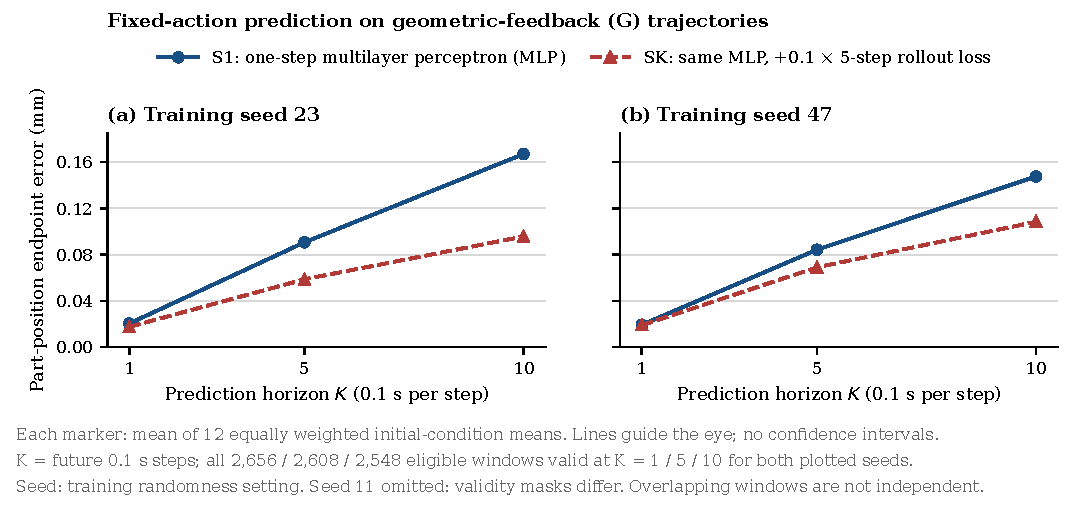
\includegraphics[width=\textwidth]{fixed_prediction.pdf}
\caption{고정 G 행동에서 seed23·47의 길이별 위치오차.
두 seed의 S1/SK는 모든 실제 적격 창에서 예측이 유효했다.
각 점은 12개 family 평균을 동일 가중 평균한 기술 통계이며 독립 반복의 신뢰구간이 아니다.
G 경로의 분포는 자체 정책이 폐루프에서 방문하는 상태 분포와 다르다.}\label{fig:prediction}
\end{figure*}

\subsection{후보 선택}
E1의 family 우선 평균 선택손실은 R 10.486563, S1 6.612161, SK 6.618703이었다.
SK--S1 차이는 $+0.006542$, 95\% 구간은 $[0,+0.013085]$다.
S1--R과 SK--R 차이는 각각 $-3.874402$, $-3.867860$이고,
구간 $[-12.993695,5.244890]$, $[-12.993695,5.257975]$가 0을 포함한다.
84개 집합 모두 손실이 정의되었고 선택 후보의 실제 무효는 없었다.
사후 분석에서 동일 seed·상태 36쌍 중 35쌍은 같은 후보를 골랐다.
유일한 차이는 병진 첫 family의 G tick29, seed47이었다.
S1은 후보2·손실0, SK는 후보6·손실0.235521이었다.
이는 G 경로 N16/H5에 한정되며 온라인 N128 정책 전체가 같다는 뜻은 아니다.

\subsection{폐루프 인계}
표~\ref{tab:handoff}는 성공과 실패 포함 끝점 평균, 표~\ref{tab:strata}는 층별 성공이다.
G의 관측 성공률이 가장 높았으나 4/12는 실패했다.
S1 seed별 성공은 4/12·5/12·4/12이고 SK는 모두 4/12였다.
회전 층의 학습 계획기 비율은 G보다 높지만 층당 독립 조건은 4개뿐이다.

\begin{table}[t]
\caption{폐루프 인계 및 실패 포함 끝점 평균.
S1/SK 독립 family는 12개이며 36회는 seed 조합 수다.}\label{tab:handoff}
\centering\small
\begin{tabular}{@{}lrrrr@{}}
\toprule 방법 & 성공/$N$ & 위치(mm) & 방향($^\circ$) & 종료(s)\\ \midrule
G & 8/12 & 5.787 & 1.044 & 22.133\\
R & 0/12 & 17.102 & 8.074 & 30.000\\
S1 & 13/36 & 9.683 & 3.033 & 20.972\\
SK & 12/36 & 11.492 & 2.728 & 21.939\\
\bottomrule
\end{tabular}
\end{table}

\begin{table}[t]
\caption{층별 인계 성공}\label{tab:strata}
\centering\small
\begin{tabular}{@{}lrrr@{}}
\toprule 방법 & 병진 & 회전 & 오프셋\\ \midrule
G & 4/4 & 1/4 & 3/4\\
R & 0/4 & 0/4 & 0/4\\
S1 & 7/12 & 6/12 & 0/12\\
SK & 6/12 & 6/12 & 0/12\\
\bottomrule
\end{tabular}
\end{table}

짝비교는 표~\ref{tab:paired}와 같다.
MLP는 R보다 많은 성공을 기록했으나 SK의 S1 대비 개선은 확인되지 않았다.
0을 포함한 구간은 동등성 증거가 아니다.
Seed23의 SK K5 오차는 0.090605에서 0.058647\,mm로 낮았으나 성공은 5/12에서 4/12로 감소했다.
Seed47은 0.084235에서 0.068994\,mm로 낮았지만 성공은 모두 4/12였다.

\begin{table}[t]
\caption{짝비교 성공 차이 (percentage points).
12개 독립 family의 층화 bootstrap; 탐색적 비교.}\label{tab:paired}
\centering\small
\begin{tabular}{@{}lrr@{}}
\toprule 비교 & 차이 & 95\% 구간\\ \midrule
R--G & $-66.67$ & $[-83.33,-50.00]$\\
S1--G & $-30.56$ & $[-63.89,2.78]$\\
SK--G & $-33.33$ & $[-66.67,0.00]$\\
S1--R & $+36.11$ & $[16.67,58.33]$\\
SK--R & $+33.33$ & $[8.33,58.33]$\\
SK--S1 & $-2.78$ & $[-8.33,0.00]$\\
\bottomrule
\end{tabular}
\end{table}

\subsection{실패 유형}
96개 종료는 ready33, timeout59, 제어 불가1, 계획 무효3이다.
실패63개에서 위치 조건 미충족62개, 방향38개, 각속도2개, 선속도0개를 관찰했다(중복 집계).
이는 증상이며 오차의 인과 원인을 식별한 수치가 아니다.
G의 한 회전 실행은 위치4.954\,mm·방향$0.119^\circ$와 두 속도 조건을 만족했으나 유지0.0825\,s로 실패했다.
S1의 오프셋3실행은 128개 후보가 모두 예측 침투 검사에서 거절됐다.
그 실패 상태에서 후보들의 실제 미래를 실행하지 않았으므로 물리적으로 복구 불가능했다고 해석하지 않는다.
G의 제어 불가는 제한된 접촉면의 복구 방향을 만들지 못한 사례였다.

\section{논의}\label{sec:discussion}
\subsection{확인된 연결과 원인 가설}
관찰은 세 수준으로 나뉜다.
일부 seed의 고정 행동 예측은 개선되었고, E1의 선택은 대부분 같았으며, 최종 SK 인계 개선은 확인되지 않았다.
후보 순위의 여유, 오류의 상태·성분별 위치, 인계 판정의 비선형 경계가 별도 분석 대상임을 시사한다.
그러나 선택 일치만으로 비용이 둔감하다고 확정할 수는 없다.
모델 예측이 유사했거나 후보군이 개선을 드러내지 못했을 수도 있다.
G 경로와 자체 정책의 방문 분포는 다르지만 그 차이의 인과 기여도는 측정하지 않았다.
H5·단일 접촉면·고정 후보 생성도 복구를 제한할 수 있으나 같은 실패 상태에서 모델 오류와 탐색 제약을 분리한 실험은 수행하지 않았다.
저장 E1의 오차·비용·순위 여유를 연결한 분석과 실패 직전 상태의 공통 후보 실제 대조가 후속 검증이다.

\subsection{개발 진단의 제한된 근거}
별도 H10 개발 상태에서는 실제 인계한 후보의 기존 비용9.586888이 실패 후보8.804576보다 높아 목표 불일치가 관찰되었다.
인계 우선 비용을 적용해도 실제로 인계하지 못한 다른 후보를 선택하는 예측 오류가 남았다.
해당 후보는 실제 부품 이동이 없었지만 실제 현재 상태를 다시 넣은 첫0.1\,s에서도 0.365--0.414\,mm의 이동 예측오차를 냈다.
이 국소 사례는 비용 오류와 동역학 오류가 별개일 수 있고 재귀 누적만으로 설명할 수 없는 오차가 있음을 보여준다.
자료 보완·상대위치 학습항 추가 대조에서도 일관된 개선은 확인되지 않았다.
다만 해당 자료·모델·H10 비용은 최종 H5 비교에 채택되지 않았다.
국소 개발 관찰을 최종96개 실행의 단일 원인으로 옮길 수 없으며 원문을 별도 근거로 제공한다~\cite{repository}.

\subsection{타당성의 한계}
형상·질량·마찰, 접근 접촉면과 초기조건이 제한되었다.
실물 노이즈·지연·손상·물성 변화·후속 집기·공정 처리량은 평가하지 않았다.
관측의 충분성, 모델 불확실성, 긴 계획과 다른 후보 생성의 효과도 미확인이다.
각 층의 독립 family는4개, 학습 seed는3개이며 E1은6개 독립 family의 G 경로에 한정된다.
유효 mask가 다른 예측 평균, 성공 집합이 다른 조건부 시간, 0을 포함한 구간을 일반적 우위·시간 절감·동등성으로 해석하지 않는다.
산업적 최소 의미 개선 폭도 사전에 지정하지 않았다.
결과를 범용 월드모델, 실물 개선 또는 학습 제어 전반의 우열로 확대할 수 없다.

\section{결론}\label{sec:conclusion}
한 단계와 다단계 자유 예측 학습을 통제하고 고정 행동 예측·후보 선택·폐루프 인계를 분리하여 평가하였다.
SK는 일부 공통 행동 예측에서 위치오차를 줄였으나 후보 선택손실과 인계 성공 개선은 확인되지 않았다.
35/36쌍의 선택 일치는 개선이 선택으로 전달되지 않은 지점의 근거이며, 전체 실패의 단일 원인 증거가 아니다.
후속 연구는 모델 확대에 앞서 같은 상태·후보에서 예측오차가 비용과 실제 결과에 전달되는 과정을 직접 비교할 필요가 있다.

\section*{재현성 및 도구 사용}
저장소~\cite{repository}는 코드·설정, 최종 모델7개, 정규화·준비 자료, E1/E2 선별 결과와 출처 SHA를 제공한다.
전체 고주파 원시는 공개 묶음에 포함되지 않는다.
선정33사례의 실제 제어 재실행에서 상태·명령·시각 최대 차이는0이었다.
같은 범위의 예약1조건에 8개 방법을 적용한 별도 검사에서는 G만 성공했고 E2와 합치지 않았다.
실물·OOD 일반화의 증거는 아니다.
구현·반복 실행·분석·원고 정리에 Codex를 사용했으며 생성 산출물과 수치 검산·원본 보존을 구분하였다.

\bibliographystyle{IEEEtran}
\bibliography{references}
\end{document}
